\documentclass[11pt,a4paper]{article}
\usepackage[margin=23mm]{geometry}
\usepackage[T1]{fontenc}
\usepackage{lmodern}
\usepackage{booktabs,graphicx,listings,xcolor,float,caption,amsmath,needspace}
\usepackage[hidelinks]{hyperref}
\usepackage{xurl}
\hypersetup{pdftitle={SD6103 Merged Tasks 3 and 4: 2023-2025},pdfauthor={SD6103 Project Group}}
\definecolor{codebg}{rgb}{0.97,0.97,0.97}
\definecolor{codeframe}{rgb}{0.75,0.75,0.75}
\lstset{language=SQL,basicstyle=\ttfamily\fontsize{9}{10.96}\selectfont,
 keywordstyle=\color{blue!70!black},stringstyle=\color{red!55!black},
 commentstyle=\color{gray},backgroundcolor=\color{codebg},rulecolor=\color{codeframe},
 frame=single,framerule=0.35pt,framesep=3pt,breaklines=true,breakatwhitespace=false,
 columns=fullflexible,keepspaces=true,showstringspaces=false,upquote=true,tabsize=4,
 aboveskip=7pt,belowskip=9pt,morekeywords={FILTER,WITHIN,EXTRACT,TRUE,FALSE,IS,NULLIF}}
\captionsetup{font=small,skip=7pt}
\setlength{\parindent}{0pt}
\setlength{\parskip}{5pt}
\setlength{\textfloatsep}{12pt}
\setlength{\intextsep}{12pt}
\clubpenalty=10000
\widowpenalty=10000
\raggedbottom
\setcounter{section}{4}
\begin{document}

\section{Task 4: Index Design and Experimental Evaluation}
\subsection{Objective and controlled protocol}
Task 4 selects indexes from actual EXPLAIN plans, runs each query five times on the largest Task 3 dataset, and compares indexed execution with that exact baseline. The deliverables include commented index DDL, raw observations, an Excel column chart, interpreted execution plans and reproducible scripts. This experiment uses 78,670 sales from January 2023 through December 2025; it does not mix the teammate's all-history population into the comparison.

The completed run contains 390 measured executions: 150 Task 3 baseline observations, 210 isolated candidate observations (seven configurations, six queries, five repeats), and 30 fresh confirmation observations. Each configuration has an excluded full-query warm-up and an untimed complete-result equality check. Data, SQL fingerprints, planner defaults and visibility maintenance remain unchanged. No index is forced by disabling sequential scans.

\textbf{Environment.} PostgreSQL 18.6 through PGlite 0.5.10, Node 24.22.1, Linux, Intel Xeon Platinum 8573C; nine logical CPUs are visible, while PostgreSQL parallel workers per gather are zero. Shared buffers are 128 MiB and work\_mem is 4 MiB. Storage is an in-memory WASM virtual filesystem. These actual timings are not a native PostgreSQL or physical-disk benchmark. The supplied native runner records the real server version and settings and repeats the full experiment in a new isolated schema.

\subsection{Plan-driven candidate design}
The baseline scans most transactions for Q1/Q2/Q4--Q6. Q3 filters the 3 ROOM subset twice. Q4 needs nearby rows ordered by address, distance and hawker ID. Q5/Q6 use address-centre memberships, and Q6 has a substantial grouping/sort workload. These observed operators motivate the following independent candidates.

\begin{table}[H]\centering\small
\begin{tabular}{lrrl}
\toprule
Isolated candidate & Geo. ratio & Index MiB & Used \\
\midrule
Date/type + address + lease & 0.957 & 1.875 & yes \\
Nearest-centre ordering & 1.196 & 1.570 & yes \\
3 ROOM partial covering & 1.142 & 0.766 & yes \\
4/5 ROOM partial covering & 1.001 & 2.492 & yes \\
Transaction address covering & 1.023 & 4.430 & yes \\
Reverse hawker membership & 1.032 & 1.570 & no \\
Town/address ordering & 1.002 & 0.297 & yes \\
\bottomrule
\end{tabular}
\caption{Exploratory ratio is the geometric mean of indexed/baseline mean times across Q1--Q6; below 1 is faster.}
\end{table}

The seven candidate DDL definitions are provided in \texttt{sql/05\_index\_candidates.json}; each statement has an explanatory trailing comment. Covering candidates include only projected/filter columns needed by their target queries. The 3 ROOM and 4/5 ROOM partial predicates match the corresponding query predicates. The nearest-order candidate matches Q4's deterministic ordering. The hawker-led and town-led alternatives test whether their join orders are useful rather than assuming that every foreign key needs an index for this analytical workload.

Index-only scans require both suitable index columns and visibility information. Equal VACUUM maintenance is therefore applied before baseline/index comparisons. The partial 3 ROOM trial actually uses two index-only scans with zero heap fetches, while the nearest-order trial eliminates Q4's incremental sort through an index-only scan. These plan improvements did not guarantee lower total six-query runtime in this environment. The reverse hawker index was not used. The town/address index was used but did not pass the aggregate selection criterion.

\subsection{Selection rule and confirmed index bundle}
The rule recorded before candidate evaluation retains a candidate group only when an actual plan uses one of its indexes and the equal-query-weight geometric mean ratio is below 0.98. Retained groups are recreated together and tested with five new repeats; individual gains are never added together. Only the teammate's three-index group passed the exploratory rule in this run. The fresh confirmation therefore measures precisely the following DDL.
\lstinputlisting{../evidence/run/selected_indexes.sql}

This is the confirmed experimental bundle, not a claim that three indexes are universally optimal. Within it, only \texttt{t4\_team\_month\_type} appears in the six-query plans. The address and lease indexes add storage/build/write cost without observed read benefit here. A practical deployment should test a pruned date/type-only bundle on native PostgreSQL before retaining those two unused indexes; its performance is not fabricated in this report. The selection rule evaluates candidate groups, so the measured three-index confirmation is preserved rather than silently relabelled as a one-index result.

\begin{table}[H]\centering\small
\begin{tabular}{lrrrrr}
\toprule
Query & Base mean & Base SD & Index mean & Index SD & Reduction \% \\
\midrule
Q1 & 61.13 & 3.74 & 66.59 & 4.96 & -8.93 \\
Q2 & 160.22 & 7.70 & 160.82 & 12.78 & -0.37 \\
Q3 & 43.31 & 5.89 & 31.54 & 2.25 & +27.16 \\
Q4 & 92.10 & 5.52 & 99.17 & 8.50 & -7.68 \\
Q5 & 116.93 & 15.44 & 112.19 & 7.79 & +4.05 \\
Q6 & 805.42 & 17.06 & 842.11 & 50.70 & -4.55 \\
\bottomrule
\end{tabular}
\caption{Largest-data executor times in milliseconds; five repeats and sample SD per query/configuration. Positive reduction means faster.}
\end{table}

\begin{figure}[H]\centering
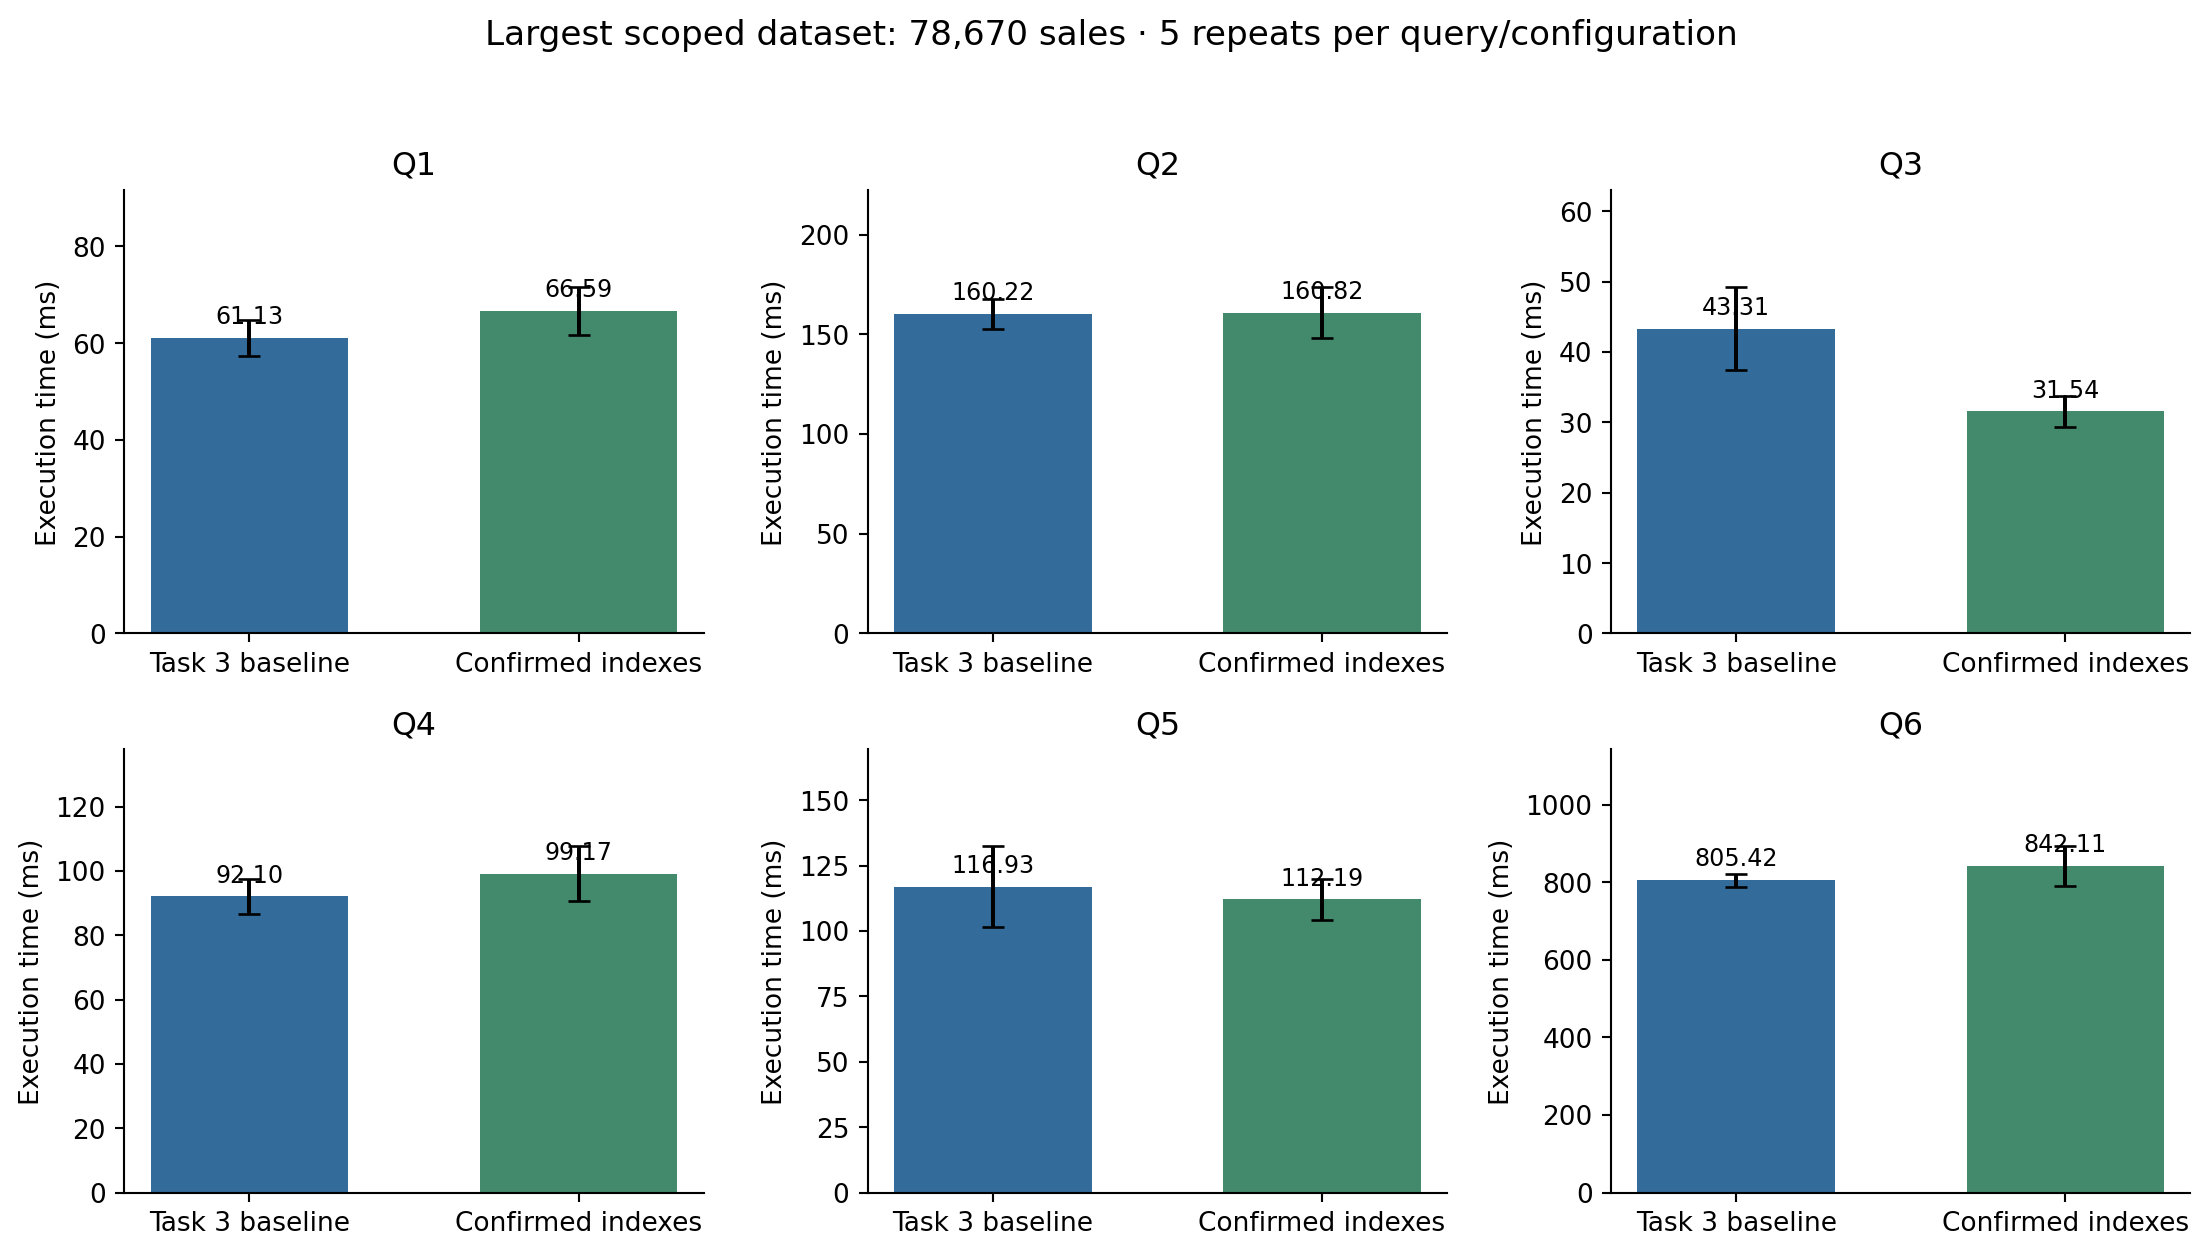
\includegraphics[width=0.95\linewidth]{../evidence/figures/Task4_comparison.png}
\caption{Task 3 S5 baseline versus the fresh confirmed bundle. Bars show means; error bars show sample SD. Every panel begins at zero.}\end{figure}
\textbf{Insight.} Q3 falls from 43.31 ms to 31.54 ms, a 27.16\% reduction. Q1, Q2, Q4 and Q6 are slower in the confirmation, while Q5 is slightly faster. The confirmation geometric mean ratio is 0.975; the sum of six mean times changes from 1279.12 to 1312.42 ms (-2.60\% reduction). The equal-query ratio suggests a modest improvement, while the sum of query means regresses; these two weightings must not be confused. This does not establish a uniformly faster workload. Five warm repeats on one host do not establish statistical significance.

\begin{table}[H]\centering\small
\begin{tabular}{lrrrrr}
\toprule
Query & Base R1 & Base R2 & Base R3 & Base R4 & Base R5 \\
\midrule
Q1 & 60.798 & 59.001 & 67.164 & 61.422 & 57.287 \\
Q2 & 165.260 & 154.585 & 171.356 & 155.590 & 154.329 \\
Q3 & 39.511 & 51.645 & 41.720 & 46.724 & 36.940 \\
Q4 & 83.462 & 93.683 & 91.356 & 98.605 & 93.414 \\
Q5 & 109.096 & 105.273 & 135.843 & 131.335 & 103.098 \\
Q6 & 805.910 & 785.182 & 829.821 & 811.689 & 794.503 \\
\bottomrule
\end{tabular}
\caption{All five raw largest-data baseline times (ms); repetition identity follows the raw CSV.}
\end{table}

\begin{table}[H]\centering\small
\begin{tabular}{lrrrrr}
\toprule
Query & Index R1 & Index R2 & Index R3 & Index R4 & Index R5 \\
\midrule
Q1 & 69.950 & 59.888 & 72.695 & 64.473 & 65.948 \\
Q2 & 163.303 & 156.445 & 180.760 & 157.555 & 146.013 \\
Q3 & 29.619 & 30.270 & 30.144 & 34.913 & 32.778 \\
Q4 & 92.233 & 98.530 & 96.049 & 113.830 & 95.229 \\
Q5 & 109.967 & 112.220 & 125.042 & 109.663 & 104.049 \\
Q6 & 805.820 & 926.672 & 834.612 & 843.220 & 800.206 \\
\bottomrule
\end{tabular}
\caption{All five raw fresh confirmation times (ms).}
\end{table}

\subsection{What the execution plans establish}
Q3's baseline scans transactions twice. The confirmed plan instead uses \texttt{t4\_team\_month\_type} bitmap index scans in both branches, each identifying 19,297 3 ROOM sales. This operator change supports the measured improvement. The date range covers all stored sales, so it is not selective; room type provides the filtering opportunity. A type-led or partial alternative remains worth testing on the intended native workload.

Q2's remaining-lease CASE expression classifies all transactions rather than searching a narrow lease interval. The lease index is unused. Q1 consumes 52,280 4/5 ROOM sales, and Q4--Q6 retain broad cohorts; none uses the confirmed optional indexes. Their output ordering and aggregates still cost work. Q4 continues to read the nearby primary-key index with an incremental sort; the separate nearest-order candidate changes that plan, but its measured total runtime does not justify claiming an overall improvement. Q6 sorts 195,690 sale-membership rows in the representative largest-data baseline. It remains dominated by membership expansion and aggregation, not a selective transaction lookup.

The relevant complete plans are stored under \texttt{evidence/run/plans}; compact node summaries and index inventories are under \texttt{evidence/run/configurations}. They record actual row counts, loops, heap fetches, buffers and sort details. A created index is considered used only when its name appears in an actual plan.

The confirmed three-index bundle occupies 1.875 MiB and takes 162.57 ms of separate build wall time in this run. Build time is not included in SELECT timings. Extra indexes also require maintenance during future inserts and updates; the read-only experiment does not quantify that write penalty.

\subsection{Deliverables and reproduction}
\texttt{SD6103\_Task4\_Results.xlsx} contains a formula-driven Summary sheet with an editable Excel bar chart, a Candidates sheet retaining all seven trials, and a Raw sheet containing all 390 observations. Means, sample deviations and reductions are calculated from raw measurements. The full raw CSV, SQL fingerprints, complete outputs, all timed plans, candidate outcomes and final index DDL accompany the workbook.

Annotated reproduction commands and dependency setup are in the package README. Both runners require an empty output folder. The native runner retains a fresh schema, repeats all trials, and selects indexes from native measurements. The macOS launcher supplies portable demo-database defaults.

\textbf{Submission boundary.} The merged queries, independent result checks and scoped WASM experiment are complete. Confirm acceptance of the 2023--2025 partition protocol and alternative tool, or run the prescribed historical-file/native procedure. Genuine pgAdmin captures must come from the native run when required; supplied figures are labelled result exports.

\subsection{References and provenance}
PostgreSQL 18 documentation: \url{https://www.postgresql.org/docs/18/sql-explain.html}; index-only scans, \url{https://www.postgresql.org/docs/18/indexes-index-only-scans.html}; partial indexes, \url{https://www.postgresql.org/docs/18/indexes-partial.html}.

Teammate source: \url{https://github.com/yzxfwdplf/SD6103-Data-Systems-Task3}. The archived snapshot records file-level blob SHAs and URLs, with the root tree labelled separately. Uploaded SQL, scoped-data manifests and validation evidence are preserved in the package.

\end{document}
